\newpage
\subsection{Method Signatures}
\texHeader
\hypertarget{static:methods tex}{}

\begin{itemize}
  
\item[$\blacktriangleright$] We're nearing the end of our model creation! One of the last things we need to do is to make the program \emph{do} something. After
all, what good is a program that only stores attributes and references?

\item[$\blacktriangleright$] In a language, the rules that describe a system's behavior - how it evolves over time or reacts to external stimulus - are
collectively referred to as \emph{Dynamic Semantics}\marginpar{\emph{Dynamic Semantics}}. Although these could be defined as a separate set of \emph{model
transformations}, we take a holistic approach and advocate integrating these transformations directly in the metamodel as operations. This naturally falls
within the OO paradigm in many ways.

\item[$\blacktriangleright$] Lets start to set up our these operations by declaring their \emph{signatures}, starting with the \texttt{Partition} class. We want
a partition to be able to do three things: compare the answer on a \texttt{card} with a guess and return a true/false value, remove a specific card, or empty
itself of all cards to reset.

\item[$\blacktriangleright$] Start with the \texttt{empty} method - it won't need any parameters, and it doesn't need to return anything. Declare this via a
\texttt{empty():void} command\footnote{If you're having difficulty remembering the syntax for MOSL, feel free to review \mbox{\texttt{Part I}}} .

\item[$\blacktriangleright$] Create two more functions for \texttt{Partition} the same way. We'll need a \texttt{removeCard} method that accepts and returns a
\texttt{Card}, as well as a EBoolean \texttt{check} method that accepts a \texttt{Card} and an \texttt{EString} guess. Your partition class should now resemble
Fig.~\ref{fig:partitionMethods}.

\begin{figure}[htbp]
	\centering
  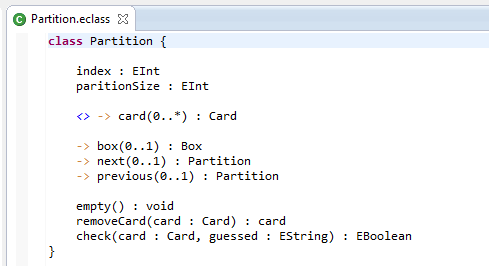
\includegraphics[width=0.6\textwidth]{eclipse_partitionMethods}
	\caption{The completed \texttt{Partition} class}
	\label{fig:partitionMethods}
\end{figure}

\item[$\blacktriangleright$] What needs to be done in the \texttt{Card} class? Well, in order to check the card, we'll need to be able to look at the flip side.
We'll also need to print whatever is on the current side. Create two void functions, \texttt{invert} and \texttt{printCard}.

\item[$\blacktriangleright$] Finally, what do we need to do with the largest object in our model, the \texttt{Box}? In summary, we want a \texttt{Box} to:

\begin{description}
	{\small
  \item[\texttt{determineNextSize():EInt }] find out how large the upcoming partition is
  \item[\texttt{grow():void}] increase in size to allow more partitions
  \item[\texttt{toString():EString}] put all box contents to a string \ldots
  \item[\texttt{addToStringRep(card:Card):void}] \ldots so we can represent them as a string
  }
\end{description}


\item[$\blacktriangleright$] Your workspace should now resemble figure~\ref{fig:workspaceMethods}.
\begin{figure}[htbp]
	\centering
  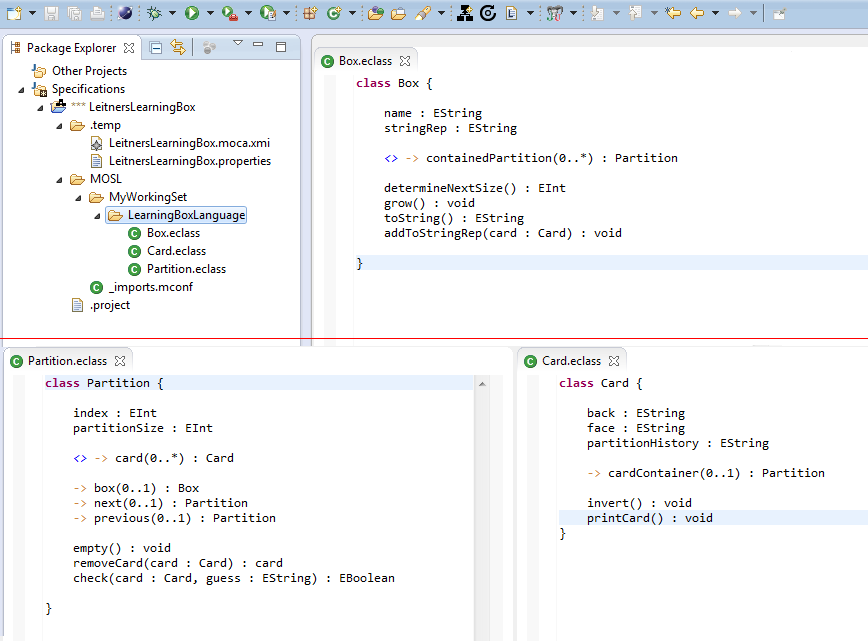
\includegraphics[width=0.95\textwidth]{eclipse_workspaceMethods}
	\caption{Completed method signatures}
	\label{fig:workspaceMethods}
\end{figure}


Congratulations! You've \emph{almost} completeley modeled Leitner's Learning Box using a concrete, textual syntax! To see how this looks in visually in a class
diagram, check out Fig.~\ref{fig:metamodel_complete} from \hyperlink{sec:static vis}{section 2.1}.

\item[$\blacktriangleright$]The very last thing we need to do is conduct a build and generate the required \texttt{.genmodel} and \texttt{.ecore} files. Beside
the \texttt{New Metamodel} button on the toolbar, you'll notice that there is a circular arrow button that offers to ``Build (without cleaning).''   %explain
this here? Press it, and wait for the package explorer to refresh.

\item[$\blacktriangleright$] If you've done everything correctly, a new \texttt{MyWorkingSet} node should have appeared, and your entire expanded explorer
should resemble Fig.~\ref{fig:builtModel}.

\begin{figure}[htbp]
	\centering
  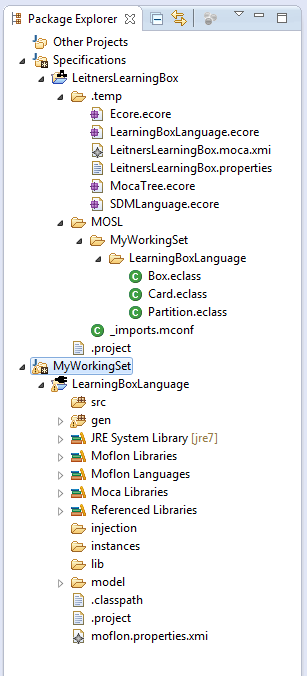
\includegraphics[width=0.5\textwidth]{eclipse_finalPackageExplorer}
	\caption{Final project structure of our Static Semantics}
	\label{fig:builtModel}
\end{figure}

\item[$\blacktriangleright$] Examine the generated files in \texttt{gen} folder, especially the default implementation for all methods that just throw an
\texttt{OperationNotSupported} exception. We shall see in later parts of this handbook that the EMF code generator actually supports injecting hand-written
implementation of methods into generated methods and classes. With eMoflon however, we can model a large part of the dynamic semantics with ease, and only need
to implement small helper methods (such as those for string manipulation) by hand.

\item[$\blacktriangleright$] Finally, you can see that your two metamodels have been created and placed in the \texttt{model} folder. Together, they form
everything the EMF needs to generate your program. If you like, instead of viewing your \texttt{.ecore} model in a tree diagram, you can request eclipse to
build a visual diagram with its built-in visual modeler! Right click on \texttt{LearningBoxLanguage.ecore} and select ''Initilalize Ecore Diagram File.''

\fancyfoot[R]{ $\triangleright$ \hyperlink{static review}{Next}}

\item[$\blacktriangleright$] You're all done! We encourage you to review the identical program construction using eMoflon's visual tools in
\hyperlink{sec:static vis}{section 2.1}, and observe how this same project is crafted using diagrams. Compare the differences between modeling the three classes in a
separate, abstract program and exporting to eclipse in order to build them, versus modeling and building all within eclipse. Which do you find easier to work
with?

\end{itemize}